\let\negmedspace\undefined
\let\negthickspace\undefined
\documentclass[journal]{IEEEtran}
\usepackage[a5paper, margin=10mm, onecolumn]{geometry}
%\usepackage{lmodern} % Ensure lmodern is loaded for pdflatex
\usepackage{tfrupee} % Include tfrupee package

\setlength{\headheight}{1cm} % Set the height of the header box
\setlength{\headsep}{0mm}     % Set the distance between the header box and the top of the text

\usepackage{gvv-book}
\usepackage{gvv}
\usepackage{cite}
\usepackage{amsmath,amssymb,amsfonts,amsthm}
\usepackage{algorithmic}
\usepackage{graphicx}
\usepackage{textcomp}
\usepackage{xcolor}
\usepackage{txfonts}
\usepackage{listings}
\usepackage{enumitem}
\usepackage{mathtools}
\usepackage{gensymb}
\usepackage{comment}
\usepackage[breaklinks=true]{hyperref}
\usepackage{tkz-euclide} 
\usepackage{listings}
                                         
\def\inputGnumericTable{}                                 
\usepackage[latin1]{inputenc}                                
\usepackage{color}                                            
\usepackage{array}                                            
\usepackage{longtable}                                       
\usepackage{calc}                                             
\usepackage{multirow}                                         
\usepackage{hhline}                                           
\usepackage{ifthen}                                           
\usepackage{lscape}
\begin{document}


\bibliographystyle{IEEEtran}

\title{5.8.19}
\author{EE25BTECH11021 - Dhanush sagar}
% \maketitle
% \newpage
% \bigskip
\maketitle \vspace{-1cm}
\renewcommand{\thefigure}{\theenumi}
\renewcommand{\thetable}{\theenumi}
\setlength{\intextsep}{10pt} % Space between text and floats

\
\numberwithin{figure}{enumi}
\renewcommand{\thetable}{\theenumi}

\textbf{Question:}  \\
If we add 1 to the numerator and subtract 1 from the denominator, a fraction reduces
to 1. It becomes 1/2 if we only add 1 to the denominator. What is the fraction?


\textbf{Solution:}


Let the unknown fraction be represented as
\begin{align}
\vec{u} &= \myvec{x \\ y}, \qquad 
\frac{x}{y}.
\end{align}

Affine transformations are written as a vector plus a translation.\\

case 1:add 1 to numerator, subtract 1 from denominator
\begin{align}
T_1(\vec{u}) &= \vec{u} + \myvec{1 \\ -1}, \quad 
\end{align}

case 2:add 1 to denominator
\begin{align}
T_2(\vec{u}) &= \vec{u} + \myvec{0 \\ 1}, \quad
\end{align}

Condition for a fraction:  
For any vector $\myvec{a \\ b}$, the requirement $\tfrac{a}{b}=k$ is equivalent to the linear equation
\begin{align}
\vec{r}_k \myvec{a \\ b} = 0, 
\qquad \vec{r}_k = \myvec{1 & -k},
\end{align}
since $\vec{r}_k \myvec{a \\ b} = a - kb = 0 \iff \tfrac{a}{b}=k$.



Case 1: $T_1(\vec{u})$ must yield fraction $1$.use $\vec{r}_1 = \myvec{1 & -1}$
\begin{align}
\vec{r}_1 \big(T_1(\vec{u})\big) &= 0 \\
\implies \vec{r}_1\vec{u} + \vec{r}_1\myvec{1 \\ -1} &= 0 \\
\myvec{1 & -1}\vec{u} + 2 &= 0 
\end{align}
This gives the first equation.



Case 2: $T_2(\vec{u})$ must yield fraction $\tfrac{1}{2}$.  
To avoid fractions, multiply the functional by $2$, i.e., use $\vec{r}_2 = \myvec{2 & -1}$.
\begin{align}
\vec{r}_2 \big(T_2(\vec{u})\big) &= 0 \\
\implies \vec{r}_2\vec{u} + \vec{r}_2\myvec{0 \\ 1} &= 0 \\
\myvec{2 & -1}\vec{u} - 1 &= 0 
\end{align}
This gives the second equation.



System of equations:  
Both conditions together form the system
\begin{align}
\myvec{1 & -1 \\ 2 & -1}\vec{u} &= \myvec{-2 \\ 1}.
\end{align}



Gaussian elimination:  
Form the augmented matrix
\begin{align}
\left[\myvec{1 & -1 \\ 2 & -1} \;\middle|\; \myvec{-2 \\ 1}\right].
\end{align}
Eliminate the entry below the pivot:
\begin{align}
R_2 \leftarrow R_2 - 2R_1 \;\;\Rightarrow\;\;
\left[\myvec{1 & -1 \\ 0 & 1} \;\middle|\; \myvec{-2 \\ 5}\right].
\end{align}
Now eliminate above the pivot:
\begin{align}
R_1 \leftarrow R_1 + R_2 \;\;\Rightarrow\;\;
\left[\myvec{1 & 0 \\ 0 & 1} \;\middle|\; \myvec{3 \\ 5}\right].
\end{align}



Final solution:
\begin{align}
\vec{u} &= \myvec{3 \\ 5}, \\
\frac{x}{y} &= \frac{3}{5}.
\end{align}

\begin{figure}[H]
    \centering
    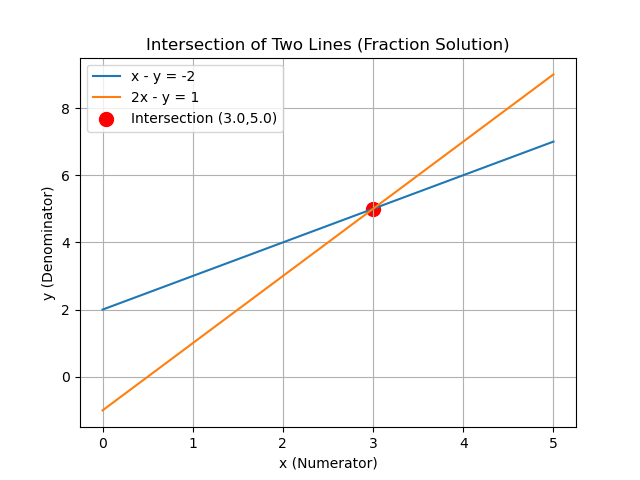
\includegraphics[width=0.5\columnwidth]{figs/fig1.png}
    \caption{}
    \label{fig:placeholder}
\end{figure}





\end{document}